\documentclass[../../main.tex]{subfiles}

\graphicspath{{../../image/}{../../figure/}}

\begin{document}

在讨论多项式曲线拟合时，我们引入了正则化的概念，其通过防止模型参数取值过大来减少过拟合（参见\cref{subsection:ch01-正则化}）。这涉及向误差函数中添加一个简单的惩罚项，从而得到正则化的误差函数，形式如下：
\begin{align}
\widetilde{E}(\boldsymbol{w}) = E(\boldsymbol{w}) + \frac{\lambda}{2}\boldsymbol{w}^{\mathsf T}\boldsymbol{w},
\label{align:ch09-正则化误差}
\end{align}
其中 $\boldsymbol{w}$ 是模型参数向量，$E(\boldsymbol{w})$ 是未正则化的误差函数，正则化超参数 $\lambda$ 控制正则化效应的强度。在以增加一些偏差为代价的情况下减小解的方差可以改善预测准确性，这可以从偏差--方差权衡的角度来解释（参见\cref{section:ch04-偏差方差权衡}）。在本章中，我们将深入探讨正则化，并讨论几种不同的正则化方法。我们还将看到，能从有限训练数据集中获得良好泛化能力的偏差所起的重要作用。

\begin{definition}[正则化误差函数]\label{definition:ch09-正则化误差函数}
设 $E(\boldsymbol{w})$ 是模型参数 $\boldsymbol{w}\in\mathbb{R}^{M}$ 的未正则化误差函数，$\lambda\geqslant0$ 是正则化超参数。称由\eqref{align:ch09-正则化误差}定义的 $\widetilde{E}(\boldsymbol{w})$ 为\textbf{正则化误差函数}（regularized error function），称 $\frac{\lambda}{2}\|\boldsymbol{w}\|^{2}$ 为\textbf{正则化项}（regularization term）或\textbf{惩罚项}（penalty term），$\lambda$ 为\textbf{正则化系数}（regularization coefficient）。当 $\lambda=0$ 时正则化误差函数退化为原来的误差函数 $E(\boldsymbol{w})$。
\end{definition}

% SUPPLEMENT: parent=definition:ch09-正则化误差函数; kind=motivation; location=紧随其后的 remark（重构新增）
\begin{remark}（重构新增）\cref{definition:ch09-正则化误差函数}把“防止参数过大”这一直观要求写成可优化的目标：在原有误差 $E$ 上加一项只依赖于参数大小的惩罚。因子 $1/2$ 只是为了让求导后的系数为 $1$（见\cref{align:ch09-权重衰减梯度}），不影响最优解的位置。$\lambda$ 的作用是双重的：$\lambda\to0$ 时惩罚消失，模型退化为最大似然/最小二乘解，方差大而偏差小；$\lambda\to\infty$ 时最优解被压向 $\boldsymbol{w}=\boldsymbol{0}$，偏差大而方差小。因此 $\lambda$ 并不是“越大约好”或“越小越好”的固定选择，而是控制有效模型复杂度的连续旋钮，需要由验证集或 Bayes 证据确定。二次惩罚之所以常用，一是它可微且导数线性，二是它等价于零均值 Gauss 先验的负对数（见\cref{proposition:ch09-Gauss先验}），从而把“偏好小参数”这一归纳偏置纳入概率框架。
\end{remark}

在实际应用中，产生数据的过程不太能够精确对应于特定的神经网络架构，因此任何给定的神经网络都只是对真实数据生成器的一种近似。更大的网络可以提供更接近的近似，但这会带来过拟合的风险。实践中我们发现，最佳的泛化结果几乎总是通过使用较大的网络结合某种形式的正则化来获得的。在本章中，我们将探索几种可替代的正则化技术，包括早停法、模型平均、dropout、数据增强和参数共享。如果需要，也可以结合使用多种正则化技术。例如，正则化的误差函数［\eqref{align:ch09-正则化误差}］通常可以与 dropout 一起使用。

\section{归纳偏置}\label{section:ch09-归纳偏置}

在比较正弦合成数据问题中各阶多项式的预测误差时（参见\cref{subsection:ch01-模型复杂度}），我们发现使用中等复杂度的多项式能够获得最小的泛化误差，既不过于简单也不过于灵活。当使用形如\eqref{align:ch09-正则化误差}的正则化项来控制模型复杂度时，我们也发现了类似的结果：当正则化系数 $\lambda$ 大小中等时，我们实现了对新输入值的最佳预测（参见\cref{subsection:ch01-正则化}）。

对这一结果的洞察来自偏差--方差分解。我们看到，模型中适当的偏差水平对于从有限数据集中学习泛化能力是比较重要的（参见\cref{section:ch04-偏差方差权衡}）。具有高偏差的简单模型无法捕捉到潜在数据生成过程中的变化，而具有低偏差的高度灵活模型则容易过拟合，导致泛化能力差。随着数据集大小的增加，我们可以使用具有更小偏差的更灵活的模型，而不会引起过大的方差，从而改善泛化能力。请注意，在实际设置中，模型的选取也可能受到内存使用或执行速度等因素的影响。在此我们忽略这些附加因素，而专注于实现良好的预测性能，也就是良好的泛化能力。

\subsection{逆问题}\label{subsection:ch09-逆问题}

模型选择问题是机器学习的核心，可以追溯到大多数机器学习任务都是\textbf{逆问题}（inverse problem）这一事实。给定条件分布 $p(t\mid\boldsymbol{x})$ 以及一组有限的输入点 $\{\boldsymbol{x}_{1},\cdots,\boldsymbol{x}_{N}\}$，原则上至少可以从该分布中抽样相应的值 $\{t_{1},\cdots,t_{N}\}$。然而，在机器学习中，我们必须解决这个问题的逆问题，即只给定有限数量的样本就推断整个分布。这本质上是不适定的（ill-posed），因为有无限多的分布可能生成我们所观测到的训练数据。实际上，任何在观测目标值上具有非零概率密度的分布都是候选分布。

\begin{definition}[逆问题与不适定性]\label{definition:ch09-逆问题}
设条件分布 $p(t\mid\boldsymbol{x})$ 生成有限样本 $\{(\boldsymbol{x}_{n},t_{n})\}_{n=1}^{N}$。由有限样本推断 $p(t\mid\boldsymbol{x})$（或更一般地，由观测结果反推生成机制、由输出反推输入）的任务称为\textbf{逆问题}（inverse problem）。若该问题的解不唯一，或解不连续依赖于观测数据（观测的微小扰动可导致解的剧烈变化），则称它是\textbf{不适定的}（ill-posed）。
\end{definition}

% SUPPLEMENT: parent=definition:ch09-逆问题; kind=motivation; location=紧随其后的 remark（重构新增）
\begin{remark}（重构新增）\cref{definition:ch09-逆问题}中的两个“不”对应 Hadamard 意义下适定性的三条要求（解存在、唯一、稳定）中后两条的失效。这里的困难不是数值算法不够好，而是问题本身的信息不足：给定 $N$ 个样本点，任何在这些点上与观测目标值吻合、而在其余点任意取值的分布都与数据相容，候选集合因此是无限维的。正因如此，学习算法必须额外引入选择准则；这个准则就是下一小节定义的归纳偏置。反过来，适定的正问题（由分布生成样本）在计算上也可能很难，但那属于采样与数值计算问题，与这里讨论的“解不唯一”不是一回事。
\end{remark}

然而，为了使机器学习有实用价值，我们需要对新的 $\boldsymbol{x}$ 值进行预测，因此需要一种方法来从无限多可能分布中选择一个特定的分布。选择这个特定分布而非其他分布的偏好称为\textbf{归纳偏置}（inductive bias）或\textbf{先验知识}（prior knowledge），其在机器学习中起着核心作用。

\begin{definition}[归纳偏置]\label{definition:ch09-归纳偏置}
在从与训练数据相容的无限多个候选分布（或候选函数）中选择一个特定分布（或函数）时，所采用的、不依赖于具体训练样本的偏好，称为\textbf{归纳偏置}（inductive bias）。当这种偏好以关于问题领域的背景知识的形式给出时，也称为\textbf{先验知识}（prior knowledge）。
\end{definition}

% SUPPLEMENT: parent=definition:ch09-归纳偏置; kind=motivation; location=紧随其后的 remark（重构新增）
\begin{remark}（重构新增）\cref{definition:ch09-归纳偏置}强调“不依赖于具体训练样本”：归纳偏置是学习算法在见到数据之前就带有的选择倾向，而不是从数据中估计出来的量。它可以是显式的（如\eqref{align:ch09-正则化误差}的二次惩罚、\cref{definition:ch09-群}所刻画的对称性约束），也可以是隐式的（如网络层数、卷积的局部连接、参数初始化）。没有归纳偏置就无法从有限数据中泛化：训练集上完全拟合的函数有无穷多个，算法必须靠某种偏好挑出一个。但偏置也不是越多越好——若偏置与真实数据生成过程不一致，再多的数据也无法弥补系统性偏差。下一小节的无免费午餐定理正是这一点的极端表述。
\end{remark}

先验知识可能来自有助于约束解空间的背景信息。对于许多应用，输入值的微小变化应该导致输出值的微小变化，因此应该使解偏向于那些具有平滑变化函数的解决方案。形如\eqref{align:ch09-正则化误差}的正则化项鼓励模型权重取值较小，因此引入了对输入变化较慢的函数的偏好。同样，当我们在图像中检测对象时，可以利用对象本体通常与对象在图像中的位置无关的先验知识（参见\cref{chapter:ch10-卷积网络}）。这称为\textbf{平移不变性}（translation invariance），将其纳入我们的解可以显著简化构建具有良好泛化能力的系统的任务。然而，必须注意不要引入与数据生成过程不一致的偏差或约束。例如，当输出与输入之间实际存在显著的非线性关系时，如果假设它们的关系是线性的，则可能导致得到一个产生不准确答案的系统。

像迁移学习和多任务学习这样的技术也可以从正则化的角度来看（参见\cref{subsection:ch06-迁移学习}）。当某个特定任务的训练数据有限时，可以使用来自不同但相关任务的额外数据来帮助确定神经网络中的可学习参数。任务之间的相似性假设代表了一种比简单正则化更复杂的归纳偏置形式，这解释了使用额外数据所带来的性能提升。

\subsection{无免费午餐定理}\label{subsection:ch09-无免费午餐}

本书的核心关注点是一类重要的机器学习模型——深度神经网络。这些模型高度灵活，并已经在计算机视觉、语音识别和自然语言处理等多个领域引发了革命。事实上，它们已成为大多数机器学习应用的首选框架。因此，它们看起来像是能完成所有任务的“通用”学习算法。然而，即便是非常灵活的神经网络也包含重要的归纳偏置（参见\cref{chapter:ch10-卷积网络}）。例如，卷积神经网络编码了特定形式的归纳偏置，包括对图像应用特别有用的平移不变性。

\textbf{无免费午餐定理}（no free lunch theorem）（Wolpert，1996）源自“天下没有免费的午餐”这一说法，其表明在所有可能的问题上，平均来看每个学习算法与其他学习算法一样好。如果某个特定模型或算法在某些问题上优于平均水平，那么它在其他问题上必定低于平均水平。然而，这更多是一个理论概念，因为这里所说的可能问题空间，包括了在任何合理的实际应用中都非常不典型的输入与输出之间的关系。例如，我们已经注意到，大多数具有实践背景的例子显示出了某种程度的平滑性，其中输入值的微小变化大多与目标值的微小变化相关联。像神经网络这样的模型，以及大多数广泛使用的机器学习技术，由于表现出了这种形式的归纳偏置，因此在某种程度上具有广泛的适用性。

\begin{theorem}[无免费午餐定理]\label{theorem:ch09-无免费午餐}
设输入空间 $\mathcal{X}$ 与输出空间 $\mathcal{Y}$ 均为有限集，目标函数 $f:\mathcal{X}\to\mathcal{Y}$ 在全体 $|\mathcal{Y}|^{|\mathcal{X}|}$ 个函数上等可能地选取。给定训练集 $S=\{(\boldsymbol{x}_{n},f(\boldsymbol{x}_{n}))\}_{n=1}^{N}$，任一学习算法根据 $S$ 输出假设 $h_{S}:\mathcal{X}\to\mathcal{Y}$。则对任意未在训练集中出现的输入 $x_{0}\notin\{x_{1},\cdots,x_{N}\}$，该算法在 $x_{0}$ 上的期望 $0$--$1$ 误差为
\begin{align*}
\mathbb{E}_{f}\bigl[\mathbf{1}\{h_{S}(x_{0})\neq f(x_{0})\}\bigr]=\frac{|\mathcal{Y}|-1}{|\mathcal{Y}|},
\end{align*}
它与学习算法无关。
\end{theorem}

\begin{proof}
（重构新增）固定训练输入 $\{x_{1},\cdots,x_{N}\}$ 与 $x_{0}\notin\{x_{1},\cdots,x_{N}\}$。对任意与 $S$ 相容的目标函数 $f$，算法输出同一个假设 $h_{S}$，因为算法的输入只有 $S$。在全体目标函数中，与 $S$ 相容的函数共有 $|\mathcal{Y}|^{|\mathcal{X}|-N}$ 个：它们在 $N$ 个训练点上的取值已被固定，其余 $|\mathcal{X}|-N$ 个点可任意取值。其中在 $x_{0}$ 处取值不等于 $h_{S}(x_{0})$ 的函数有 $(|\mathcal{Y}|-1)|\mathcal{Y}|^{|\mathcal{X}|-N-1}$ 个：$x_{0}$ 处有 $|\mathcal{Y}|-1$ 种“错误”选择，其余 $|\mathcal{X}|-N-1$ 个点任意。由于 $f$ 等可能，所求期望误差等于上述两类函数个数之比
\begin{align*}
\frac{(|\mathcal{Y}|-1)|\mathcal{Y}|^{|\mathcal{X}|-N-1}}{|\mathcal{Y}|^{|\mathcal{X}|-N}}=\frac{|\mathcal{Y}|-1}{|\mathcal{Y}|}.
\end{align*}
该比值只依赖于 $|\mathcal{Y}|$，与 $h_{S}$ 无关，而 $h_{S}$ 是任一算法由 $S$ 产生的，故期望误差与算法无关。若算法本身带随机性，则对随机性再取一次期望，上式仍成立。
\end{proof}

% SUPPLEMENT: parent=theorem:ch09-无免费午餐; kind=motivation; location=紧随其后的 remark（重构新增）
\begin{remark}（重构新增）\cref{theorem:ch09-无免费午餐}把“平均来看每个算法一样好”精确化为：在目标函数等可能的先验下，任何算法对未见点的期望误差都等于随机猜测的误差 $(|\mathcal{Y}|-1)/|\mathcal{Y}|$。证明的关键是“算法只看到 $S$”这一信息约束——在 $x_{0}$ 处，$f$ 的取值与 $S$ 独立，算法无法提供任何信息。必须注意这个结论的适用范围：它依赖“全体函数等可能”这一极强且不现实的先验，而真实任务的目标函数高度集中（平滑、具有层次结构、满足对称性等）。因此它并不否定某个算法在特定任务上更好，而是说明“脱离任务分布的普遍最优算法”不存在；一个算法在某一类任务上的优势，必然以在另一类任务上的劣势为代价。这也解释了为什么引入与任务一致的归纳偏置（如卷积的平移等变性）能带来实际收益。
\end{remark}

尽管无免费午餐定理在某种程度上是理论性的，但它确实突出了偏差在确定机器学习算法性能方面的重要性。在没有任何偏差的情况下，不可能“纯粹从数据中”学习。在实践中，偏差可能是隐式的。例如，每个神经网络都有有限数量的参数，这限制了它所能表示的函数。然而，偏差也可以作为解决特定问题的先验知识被显式编码。

在寻找通用学习算法的过程中，我们实际上是在寻找适合的归纳偏置，它广泛适用于我们在实践中遇到的不同应用。然而，对于任何给定的应用，如果能够融入特定于该应用的更强的归纳偏置，则可以获得更好的结果。基于模型的机器学习的观点（Winn et al.，2023）主张使机器学习模型中的所有假设显式化，以便为归纳偏置做出适当的选择。

我们已经看到，可以通过分布的形式将归纳偏置融入其中，例如通过指定输出是一组基函数固定的线性函数。也可以在训练期间，通过在使用的误差函数中添加正则化项来融入归纳偏置。我们可以通过训练过程本身来控制神经网络的复杂性（参见\cref{chapter:ch07-梯度下降}）。你将看到，即使可调参数的数量超过训练数据点的数量，只要训练过程设置得当，深度神经网络也可以实现良好的泛化。将深度学习应用于现实世界问题的部分技巧在于归纳偏置的仔细设计和先验知识的融入。

\subsection{对称性和不变性}\label{subsection:ch09-对称性不变性}

在机器学习的许多应用中，预测应该在输入变量经过一种或多种变换时保持不变，称为具有\textbf{不变性}（invariance）。例如，在对二维图像中的对象进行分类时，如猫或狗，无论对象在图像中的位置如何，都应赋予对象相同的分类，称为\textbf{平移不变性}（translation invariance）。同样，图像中对象大小的变化也不应改变对象的分类，称为\textbf{尺度不变性}（scale invariance）。利用这种对称性来创建归纳偏置可以大大提高机器学习模型的性能，这是\textbf{几何深度学习}（geometric deep learning）（Bronstein et al.，2021）所要研究的主题。

\begin{definition}[不变性与对称性]\label{definition:ch09-不变性}
设 $\mathcal{T}$ 是一族作用在输入空间上的变换，$C$ 是将输入 $I$ 映射为预测 $C(I)$ 的预测器。若对每个 $T\in\mathcal{T}$ 与每个输入 $I$ 都有 $C(T(I))=C(I)$，则称 $C$ 关于 $\mathcal{T}$ 具有\textbf{不变性}（invariance）。当 $\mathcal{T}$ 为平移变换族时，称相应的不变性为\textbf{平移不变性}（translation invariance）；当 $\mathcal{T}$ 为缩放变换族时，称为\textbf{尺度不变性}（scale invariance）。若一族变换保持某个属性不变，则称该属性具有相应的\textbf{对称性}（symmetry）。
\end{definition}

% SUPPLEMENT: parent=definition:ch09-不变性; kind=motivation; location=紧随其后的 remark（重构新增）
\begin{remark}（重构新增）\cref{definition:ch09-不变性}把“对称性”从几何直观转成了对预测器的函数方程约束：对变换族中的每个 $T$，$C\circ T=C$。这一约束越强，候选函数空间越小，所需样本越少；但若真实任务并不具有该对称性（例如预测图像中对象的位置，而不是类别），强行施加不变性会丢失关键信息。平移不变性适合分类，却不适合定位与分割，这正是后文\cref{definition:ch09-等变性}要把“不变”推广为“按已知方式变换”的动机。还要注意，不变性是相对于给定的变换族而言的，脱离变换族谈“某个模型具有不变性”没有意义。
\end{remark}

平移或缩放等变换保持特定属性不变的现象称为对称性。所有对应于特定对称性（如平移或缩放）的变换的集合构成了一个称为\textbf{群}（group）的数学结构。群由一组元素 $A,B,C,\cdots$ 以及一个用于组合元素对的二元运算（使用符号 $A\circ B$ 表示）组成。以下 $4$ 个公理对于群是成立的。

\begin{definition}[群]\label{definition:ch09-群}
设 $G$ 是非空集合，$\circ:G\times G\to G$ 是定义在 $G$ 上的二元运算。若下列四条公理成立，则称 $(G,\circ)$ 为\textbf{群}（group）：
\begin{enumerate}
\item \textbf{封闭性}：对于集合中的任何两个元素 $A$ 和 $B$，$A\circ B$ 也必须在集合中；
\item \textbf{结合性}：对于集合中的任何三个元素 $A$、$B$ 和 $C$，有 $(A\circ B)\circ C=A\circ(B\circ C)$；
\item \textbf{单位元}：集合中存在一个称为单位元的元素 $I$，满足对于集合中的每个元素 $A$，有 $A\circ I=I\circ A=A$；
\item \textbf{逆元}：对于集合中的每个元素 $A$，存在集合中的另一个元素，用 $A^{-1}$ 表示，称为逆元，满足 $A\circ A^{-1}=A^{-1}\circ A=I$。
\end{enumerate}
\end{definition}

% SUPPLEMENT: parent=definition:ch09-群; kind=motivation; location=紧随其后的 remark（重构新增）
\begin{remark}（重构新增）\cref{definition:ch09-群}的作用是把“变换可以复合、可以撤销、可以什么都不做”这三件直观事情公理化。封闭性保证复合仍是允许的变换；结合性保证多步复合不必加括号；单位元对应恒等变换；逆元保证每个变换可撤销，从而变换族不会把不同的输入永久粘在一起。四条公理中，封闭性与逆元是最实质的：只满足封闭性与结合性的结构是半群，加上单位元是幺半群，只有再加上逆元才成为群。正因为有逆元，“在变换下不变”才能等价地写成“先变换再预测”与“先预测再逆变换”的一致性，这也是\cref{definition:ch09-等变性}能用 $S\circ T=\tilde T\circ S$ 表述的前提。群只刻画变换的代数结构，不涉及变换作用在具体数据上的连续性或可微性；后文的卷积网络利用的是平移群的离散版本。
\end{remark}

简单的群如以 $90^{\circ}$ 的倍数旋转正方形的变换集合，或在二维平面上连续平移对象的变换集合，都满足群公理（见\cref{exercise:ch09-01}）。

原则上，神经网络对输入空间变换做出预测的不变性可以从数据中学习，而无须对网络或训练程序进行特殊修改。然而，实际上这可能极其具有挑战性，因为这样的变换可以在原始数据中产生显著改变。例如，图像中对象的相对较小的平移，即使只有几个像素，也可以导致像素值发生显著变化。此外，多种不变性通常需要同时保持，例如同时要求对二维空间中的平移、缩放、旋转、强度变化、色彩平衡变化等保持不变。这样的变换组合的数量是指数级的，这使得学习所有这些不变性所需的训练集大得难以承受。

因此，我们需要寻求更有效的方法来促使自适应模型展现出所需的不变性。这些方法大致可以分为 $4$ 类。
\begin{enumerate}
\item \textbf{预处理}：通过在预处理阶段计算在所需变换下保持不变的数据特征来构建不变性。任何后续使用这些特征作为输入的回归或分类系统必然也保持了这些不变性。
\item \textbf{正则化的误差函数}：向误差函数中添加一个正则化项，以惩罚输入仅受不变性变换改变时模型输出的变化。
\item \textbf{数据增强}：通过使用所需的不变性对训练数据点进行变换，从而扩展训练集，同时保持它们的目标值与变换前相同。
\item \textbf{网络架构}：通过适当选择网络架构，将不变性融入神经网络的结构中。
\end{enumerate}

上述第 $1$ 类方法面临的一个挑战是设计呈现所需不变性的特征，同时不丢弃可能有助于确定网络输出的信息。我们已经看到，固定的、手工提取的特征表示能力有限，并且已被使用深度神经网络习得的表示所取代（参见\cref{chapter:ch06-深度神经网络}）。

第 $2$ 类方法的一个例子是在训练过程中添加正则化项到误差函数中的\textbf{切线传播}（tangent propagation）技术（Simard et al.，1992），旨在直接惩罚由某种不变性变换下输入变量的变化引起的输出变化。除了训练的额外复杂性外，这种技术的一个局限性是只能处理小的变换（例如少于一个像素的平移）。

第 $3$ 类方法又称\textbf{数据集增强}（data set augmentation）。它通常相对容易实现，并且在实践中被证明非常有效。它通常应用在图像分析场景中，因为创建变换的训练数据非常直接。\cref{figure:ch09-数据增强}显示了对猫的图像应用这些变换的示例。对于软组织的医疗图像，数据增强也可以包含连续的“橡皮布”变形（Ronneberger，Fischer，and Brox，2015）。

\begin{figure}[htbp]
\centering
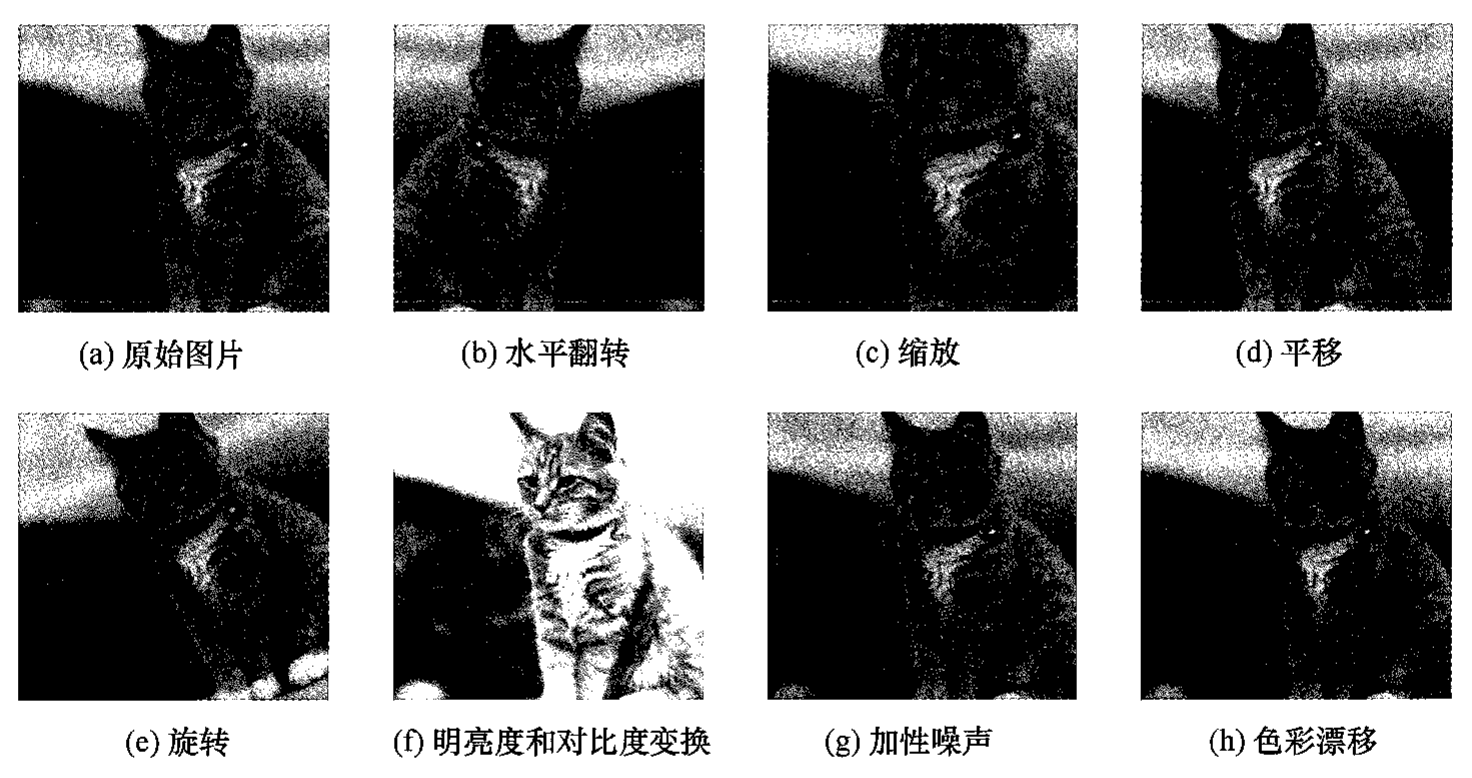
\includegraphics[width=0.95\textwidth]{ch09-fig9-1-augmentation.png}
\caption{数据集增强示意图}
\label{figure:ch09-数据增强}
\end{figure}

对于序贯训练算法，如随机梯度下降，我们可以在输入模型之前变换每个数据点来增强数据集，以便如果数据点被循环使用，则每次都会应用不同的变换（从适当的分布中抽取变换方式）。对于批训练方法，通过多次复制每个数据点并独立变换每个副本，可以达到类似的效果。

通过对原始示例做小改动的变换，然后按变换幅度的幂次对误差函数进行Taylor展开，可以分析使用增强数据的效果（Bishop，1995c；Leen，1995；Bishop，2006），并得到一个正则化的误差函数，其中的正则化项惩罚了网络输出相对于输入变量在变换方向上投影的梯度。这与前面讨论的切线传播技术相关。添加随机噪声的变换是一种特殊情况，在这种情况下，正则化项惩罚网络输出相对于输入的导数（见\cref{exercise:ch09-02}）。因为我们鼓励即便在输入变量添加噪声的情况下网络输出也保持不变，所以该惩罚是非常合理的。

最后，第 $4$ 类方法，也就是在网络结构中融入不变性，已被证明非常强大且有效，并且还带来了其他关键的好处。我们将在计算机视觉中的卷积神经网络背景下详细讨论这类方法（参见\cref{chapter:ch10-卷积网络}）。

\subsection{等变性}\label{subsection:ch09-等变性}

不变性的一个重要推广称为\textbf{等变性}（equivariance）。在这种情况下，当输入变换时，网络的输出以特定的方式变换，而不是保持不变。例如，考虑一个接收图像作为输入并返回图像分割结果的网络，其中每个像素分类为属于前景对象或背景。此时，如果图像中对象的位置发生平移，那么我们希望对象的相应分割结果也类似地发生平移。假设我们用 $I$ 表示图像，用 $S$ 表示分割网络的操作，那么对于一个平移操作 $T$，我们有
\begin{align}
S(T(I))=T(S(I)).
\label{align:ch09-等变性}
\end{align}
这表明被平移图像的分割结果是通过对原始图像的分割结果进行平移得到的。\cref{figure:ch09-等变性}说明了这种关系。

\begin{definition}[等变性]\label{definition:ch09-等变性}
设 $S$ 是将输入 $I$ 映射为输出 $S(I)$ 的算子，$\mathcal{T}$ 是作用在输入空间上的一族变换。若对每个 $T\in\mathcal{T}$ 都存在作用在输出空间上的变换 $\tilde{T}$，使得
\begin{align*}
S(T(I))=\tilde{T}(S(I))
\end{align*}
对所有 $I$ 成立，则称 $S$ 关于 $\mathcal{T}$ 是\textbf{等变的}（equivariant），$\tilde{T}$ 称为 $T$ 在输出空间的\textbf{诱导变换}。当 $\tilde{T}$ 为恒等变换时，等变性退化为不变性。
\end{definition}

% SUPPLEMENT: parent=definition:ch09-等变性; kind=motivation; location=紧随其后的 remark（重构新增）
\begin{remark}（重构新增）\cref{definition:ch09-等变性}比\cref{definition:ch09-不变性}更精细：它不要求输出“不动”，而要求输出“按与输入相同（或已知）的方式动”。这一区分对分割、检测、姿态估计等结构化输出任务是本质的——把输入图像平移几个像素，分割掩码也应相应平移，而不是保持不变。等变性的强度取决于诱导变换 $\tilde{T}$：若 $\tilde{T}=T$，称为同变；若 $\tilde{T}$ 是降采样网格上的平移，则等变性只在离散网格上近似成立。实现等变性的架构（如卷积网络对平移）把这一约束硬编码进模型，因此无需从数据中学习变换的复合规律，样本效率远高于让全连接网络自行发现。但等变性是相对于给定变换群而言的：旋转等变性需要旋转卷积或群等变网络，普通卷积并不具备。
\end{remark}

\begin{figure}[htbp]
\centering
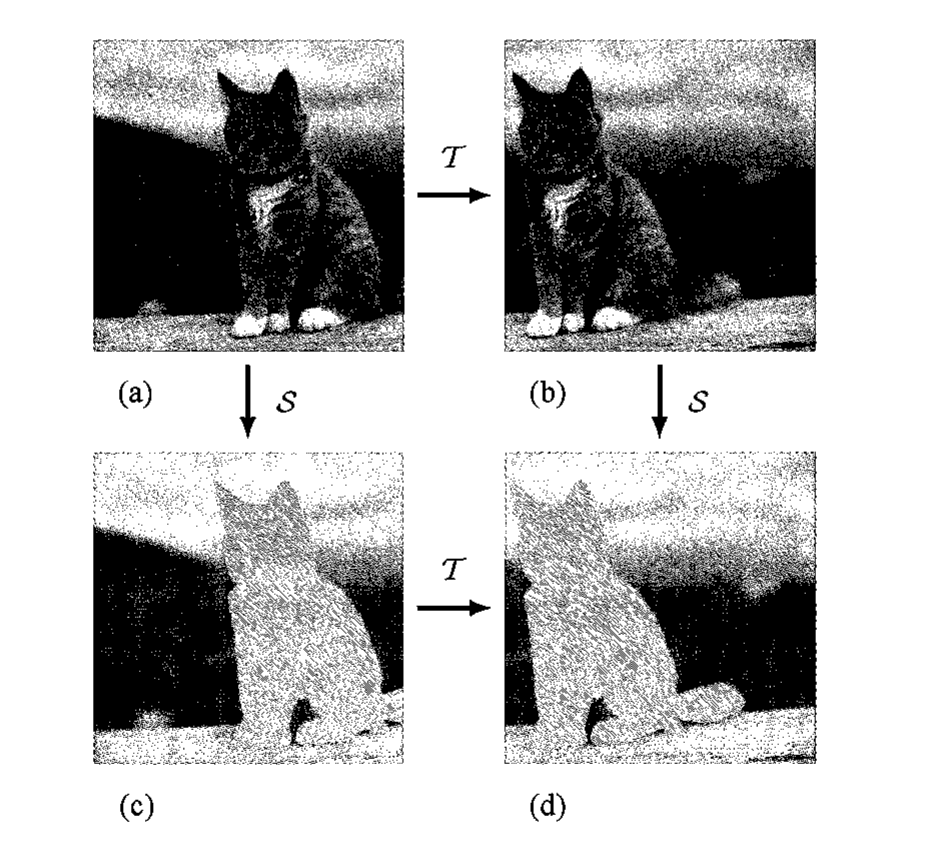
\includegraphics[width=0.55\textwidth]{ch09-fig9-2-equivariance.png}
\caption{对应\eqref{align:ch09-等变性}的等变性示意图。如果图像 (a) 首先被平移得到图像 (b)，然后被分割得到图像 (d)，则结果与先将图像 (a) 分割得到图像 (c)，再平移得到图像 (d) 相同}
\label{figure:ch09-等变性}
\end{figure}

更一般地，当应用于输出的变换与应用于输入的变换不同时，等变性也成立：
\begin{align}
S(T(I))=\tilde{T}(S(I)).
\label{align:ch09-广义等变性}
\end{align}
例如，假设分割后的图像的分辨率低于原始图像，$T$ 代表原始图像空间中的平移，$\tilde{T}$ 代表较低维度分割空间中相应的平移。同样，如果 $S$ 代表计算图像中对象方向的操作，而 $T$ 代表旋转（这是图像中所有像素值的复杂非线性变换），那么 $\tilde{T}$ 将依据 $S$ 生成一个标量方向值增大或减小。

我们还看到，不变性是等变性的一种特殊情况，其中输出变换是简单的恒等变换。例如，如果 $C$ 是一个神经网络，用于分类图像中的一个对象，而 $T$ 是一个平移操作，则有
\begin{align}
C(T(I))=C(I),
\label{align:ch09-不变性}
\end{align}
这表明对象的类别不依赖于该对象在图像中的位置。

\end{document}
